% THIS IS SIGPROC-SP.TEX - VERSION 3.1
% WORKS WITH V3.2SP OF ACM_PROC_ARTICLE-SP.CLS
% APRIL 2009
%
% It is an example file showing how to use the 'acm_proc_article-sp.cls' V3.2SP
% LaTeX2e document class file for Conference Proceedings submissions.
% ----------------------------------------------------------------------------------------------------------------
% This .tex file (and associated .cls V3.2SP) *DOES NOT* produce:
%       1) The Permission Statement
%       2) The Conference (location) Info information
%       3) The Copyright Line with ACM data
%       4) Page numbering
% ---------------------------------------------------------------------------------------------------------------
% It is an example which *does* use the .bib file (from which the .bbl file
% is produced).
% REMEMBER HOWEVER: After having produced the .bbl file,
% and prior to final submission,
% you need to 'insert'  your .bbl file into your source .tex file so as to provide
% ONE 'self-contained' source file.
%
% Questions regarding SIGS should be sent to
% Adrienne Griscti ---> griscti@acm.org
%
% Questions/suggestions regarding the guidelines, .tex and .cls files, etc. to
% Gerald Murray ---> murray@hq.acm.org
%
% For tracking purposes - this is V3.1SP - APRIL 2009

\documentclass{acm_proc_article-sp}

\usepackage{verbatim}
\usepackage{graphicx}
\usepackage{subcaption}
\usepackage{hyperref}

\begin{document}

\title{String-Embedded Language Support in Integrated Development Environment\titlenote{Permission to make digital or hard copies of all or part of this work for personal or classroom use is granted without fee provided that copies are not made or distributed for profit or commercial advantage and that copies bear this notice and the full citation on the first page. Copyrights for components of this work owned by others than ACM must be honored. Abstracting with credit is permitted. To copy otherwise, or republish, to post on servers or to redistribute to lists, requires prior specific permission and/or a fee. Request permissions from Permissions@acm.org. \\ \\CEE-SECR '14, October 23 - 25 2014, Moscow, Russian Federation \\Copyright is held by the owner/author(s). Publication rights licensed to ACM. \\ACM 978-1-4503-2889-0/14/10\$15.00 \\ \url{http://dx.doi.org/10.1145/2687233.2687247}}}

%\subtitle{[Extended Abstract]
%\titlenote{A full version of this paper is available as
%\textit{Author's Guide to Preparing ACM SIG Proceedings Using
%\LaTeX$2_\epsilon$\ and BibTeX} at
%\texttt{www.acm.org/eaddress.htm}}}
%


% You need the command \numberofauthors to handle the 'placement
% and alignment' of the authors beneath the title.
%
% For aesthetic reasons, we recommend 'three authors at a time'
% i.e. three 'name/affiliation blocks' be placed beneath the title.
%
% NOTE: You are NOT restricted in how many 'rows' of
% "name/affiliations" may appear. We just ask that you restrict
% the number of 'columns' to three.
%
% Because of the available 'opening page real-estate'
% we ask you to refrain from putting more than six authors
% (two rows with three columns) beneath the article title.
% More than six makes the first-page appear very cluttered indeed.
%
% Use the \alignauthor commands to handle the names
% and affiliations for an 'aesthetic maximum' of six authors.
% Add names, affiliations, addresses for
% the seventh etc. author(s) as the argument for the
% \additionalauthors command.
% These 'additional authors' will be output/set for you
% without further effort on your part as the last section in
% the body of your article BEFORE References or any Appendices.

\numberofauthors{5} %  in this sample file, there are a *total*
% of EIGHT authors. SIX appear on the 'first-page' (for formatting
% reasons) and the remaining two appear in the \additionalauthors section.
%
\author{
\alignauthor
Semen Grigorev\\
       \affaddr{St. Petersburg State University}\\
       \affaddr{198504, Universitetsky prospekt 28}\\
       \affaddr{Peterhof, St. Petersburg, Russia.}\\
       \email{rsdpisuy@gmail.com}
\alignauthor
Ekaterina Verbitskaia\\
       \affaddr{St. Petersburg State University}\\
       \affaddr{198504, Universitetsky prospekt 28}\\
       \affaddr{Peterhof, St. Petersburg, Russia.}\\
       \email{kajigor@gmail.com}
\alignauthor
Andrei Ivanov\\
       \affaddr{St. Petersburg State University}\\
       \affaddr{198504, Universitetsky prospekt 28}\\
       \affaddr{Peterhof, St. Petersburg, Russia.}\\
       \email{ivanovandrew2004@gmail.com}
%\additionalauthors{Additioan authors: Andrei Ivanov (St. Petersburg State University, email:{\texttt{ivanovandrew2004@gmail.com}}) and Ekaterina Mavchun (St. Petersburg State University, email:{\texttt{emavchun@gmail.com}})}
\and
\alignauthor
Marina Polubelova\\
       \affaddr{St. Petersburg State University}\\
       \affaddr{198504, Universitetsky prospekt 28}\\
       \affaddr{Peterhof, St. Petersburg, Russia.}\\
       \email{polubelovam@gmail.com}
\alignauthor
Ekaterina Mavchun\\
       \affaddr{St. Petersburg State University}\\
       \affaddr{198504, Universitetsky prospekt 28}\\
       \affaddr{Peterhof, St. Petersburg, Russia.}\\
       \email{emavchun@gmail.com}
}

%\numberofauthors{1} 
%\author{\alignauthor Semen Grigorev, Ekaterina Verbitskaia, Andrei Ivanov, Marina Polubelova, and Ekaterina Mavchun \\
%\affaddr{St. Petersburg State University}\\
%\affaddr{198504, Universitetsky prospekt 28}\\
%\affaddr{Peterhof, St. Petersburg, Russia.}
%\email{semen.grigorev@jetbrains.com, kajigor@gmail.com, ivanovandrew2004@gmail.com, polubelovam@gmail.com, emavchun@gmail.com}
%}
 
% There's nothing stopping you putting the seventh, eighth, etc.
% author on the opening page (as the 'third row') but we ask,
% for aesthetic reasons that you place these 'additional authors'
% in the \additional authors block, viz.
%\additionalauthors{Additional authors: John Smith (The Th{\o}rv{\"a}ld Group,
%email: {\texttt{jsmith@affiliation.org}}) and Julius P.~Kumquat
%(The Kumquat Consortium, email: {\texttt{jpkumquat@consortium.net}}).}
\date{10 July 2014}
% Just remember to make sure that the TOTAL number of authors
% is the number that will appear on the first page PLUS the
% number that will appear in the \additionalauthors section.

\maketitle
\begin{abstract}
Most general-purpose programming languages allow to use string literals as source code in other languages (they are named string-embedded languages). Such strings can be executed or interpreted by dedicated runtime component. This way host program can communicate with DBMS or web browser. The most common example of string-embedded language is Dynamic SQL or SQL embedded into C\#, C++, Java or other general-purpose programming languages. Standard Integrated Development Environment functionality such as syntax highlighting or static error checking in embedded languages can help developers who use such technique, but it is necessary to process string literals as a code to provide these features. We present a platform allowing to create tools for string-embedded languages processing easily, and compare it with other similar tools like IntelliLang. We also demonstrate a plug-in for ReSharper created by using the platform. The plug-in provides code highlighting and static error checking for string-embedded T-SQL in C\#.
\end{abstract}

\category{D.3.4}{Programming Languages}{Processors}[parsing]
\category{D.2.7}{Software Engineering}{Distribution, Maintenance, and Enhancement}[Restructuring, reverse engineering, and reengineering]

\terms{Algorithms, Parsing}

\keywords{String-embedded language, abstract parsing, parser generator, lexer generator, integrated development environment, IDE, Dynamic SQL.
} % NOT required for Proceedings


\section{Introduction}

Multiple languages are often used in large software system development. In this case there are one {\it host} language and one or more {\it string-embedded} or just {\it embedded} languages. String expressions of host language form programs in another language and then they are interpreted in runtime by special component such as database management system or web-browser. The majority of general-purpose programming languages can play role of both the host and the embedded programming language. Examples of embedded languages are presented below.

\begin{itemize}
%\item JavaScript code execution from Java code.

%\begin{verbatim}
%import javax.script.*;
%public class InvokeScriptFunction {
%  public static void main(String[] args) {
%    ScriptEngineManager manager = 
%      new ScriptEngineManager();
%    ScriptEngine engine = 
%      manager.getEngineByName("JavaScript");    
%    String script = 
%      "function hello(name)" +
%      "{print('Hello, ' + name);}";    
%    engine.eval(script);
%  }
%}
%\end{verbatim}
\!
\item Dynamic SQL:
\!
\begin{verbatim}
CREATE PROCEDURE [dbo].[MyProc] 
  @TBLRes   VarChar(30)
AS
  EXECUTE ('INSERT INTO ' + @TBLRes + ' (f1)'
  + ' SELECT ''Additional condition: '' + f2'
  + ' from #tt where sAction = ''100''')
GO
\end{verbatim}

\item Multiple embedded into PHP languages (MySQL, HTML):

\begin{verbatim}
<?php
  $query = 'SELECT * FROM '. $my_table;
  $result = mysql_query($query);  
  echo "<table>\n";
  while ($line = 
    mysql_fetch_array($result, MYSQL_ASSOC)){
    echo "\t<tr>\n";
    foreach ($line as $col_value) {
      echo "\t\t<td>$col_value</td>\n";
    }
    echo "\t</tr>\n";
  }
  echo "</table>\n";?> 
\end{verbatim}

\end{itemize}

String-embedded languages may help to compensate the lack of expressivity of general-purpose programming language in domain-specific settings. However, it is rather hard to develop, support or reengineer string-embedded code using this technique. Dynamically generated expression are often constructed of string primitives of the host language by concatenations in loops, conditional expressions or recursive procedures. Dynamically generated expressions are simple strings in the point of view of the host language analyser and  even syntactic analysis is undecidable in general case. Impossibility of static check for dynamic expression results in high possibility of getting errors in runtime. 


Common practice in software system development is Integrated Development Environments using that provides such features as code highlighting, autocompletion, error handling, different kinds of refactoring. All these significantly simplifies development and debugging process. Thus the tools being able to perform {\it abstract analysis}~---~static analysis of dynamically-generated expression value set~---~may be really helpful.

Grammarware research and development project YaccConst-ructor~\cite{GrigorevKirilenkoYC} is now aimed to create an infrastructure for development of string-embedded language processing tools. In this paper we provide overview of the tools for embedded languages processing, describe the infrastructure under development and its components, and pay attention to multilanguage support problems. We also describe error reporting and semantic calculation for embedded languages. Finally, we illustrate infrastructure features with developed plug-in to ReSharper\footnote{ReSharper is plug-in to Microsoft Visual Studio, extending standard IDE functionality. Site (accessed: 07.07.2014):\url{http://www.jetbrains.com/resharper/}}. 


\section{Related Work}

There are several approaches for string-embedded languages processing. The first is based on comparison of the specification of the language obtained by regular or context-free approximation of dynamically generated expression with some language reference grammar~\cite{Minamide, StringExpr}. This approach answers the question of the dynamic expression correctness, but cannot provide meaningful error report for an incorrect expression. The most languages being used as embedded are at least context free and it is rather hard to find context free grammar for them. This circumstance leads to the second drawback: low analysis precision due to the type of approximation being used.

Second approach~---~{\it abstract analysis}~\cite{LRAbstrParsing}~---~is a static analysis of some representation of dynamic expression value set. This representation can be data-flow equation, regular expression, or finite automaton~---~as it is in our platform. The tools implementing this approach can be separated into two categories: {\it analysis-and-parsing} and {\it analysis-then-parsing}. The first one stands for performing of analysis and parsing at the same time on the fly. And the second one, which is also named {\it step-by-step analysis}, means that first the analysis of source code~---~constant propagation, approximation construction~---~is performed and after that the parsing itself is executed. We use step-by-step analysis in our framework.


\subsection{Existing Tools}

There are several tools for processing of concrete string-embedded languages. They differ in the approaches used and the ease of new language extension support. We provide a brief overview of these tools below. \newline



\subsubsection{PhpStorm}

PhpStorm\footnote{IDE for PHP programming language. Site (accessed: 07.07.2014): \url{http://www.jetbrains.com/phpstorm/}}~---~integrated development environment for PHP which implements code highlighting and autocompletion of string-embedded HTML, CSS, JavaScript or SQL code. However, only if the tool deals with string primitive (no string operation is used for expression construction), it is able to provide this support. You can see PhpStorm screenshot that illustrates this feature in figure~\ref{PHPStorm}. \verb|"."| is concatenation operator and \verb|".="| is concatenating assignment operator. As you can see, PhpStorm recognises \verb|$hello| value as HTML expression and provides code highlighting, but no highlighting is performed for \verb|$string| values. PhpStorm provides a separate code editor for every string-embedded language. The drawback is that the tool does not provide error reporting for incorrect expressions (see \verb|$error| in figure~\ref{PHPStorm}).


\begin{figure}[h!]
    \begin{center}
        \includegraphics[scale=0.30]{graphics/PHPStorm.png}
    \end{center}
    \caption{HTML code embedded in PHP code in PHPStorm}
    \label{PHPStorm}
\end{figure} 

\subsubsection{IntelliLang}

IntelliLang\footnote{IntelliLang is a plug-in offering a number of features related to the processing of embedded languages. Site (accessed: 07.07.2014): \url{ http://www.jetbrains.com/idea/webhelp/intellilang.html}}~---~plug-in to PhpStorm IDE and IntelliJ IDEA\footnote{IntelliJ IDEA is an IDE for JVM-based development. Site (accessed: 07.07.2014): \url{http://www.jetbrains.com/idea/}} performing code highlighting and error reporting for string-embedded languages. It provides a separate code editor for embedded language processing by analogy with PhpStorm. The screenshots of IntelliLang are presented in figures~\ref{error_IDEA} and~\ref{IDEA_html}.

\begin{figure}[h!]
    \begin{center}
        \includegraphics[scale=0.3]{graphics/error_IDEA.png}
    \end{center}
    \caption{Embedded Java code fragment in IntelliJ IDEA}
    \label{error_IDEA}
\end{figure} 

The drawback of the plug-in is that it is necessary to specify manually the language of every string expression to be analysed. Figure~\ref{IDEA_html} illustrates the drawback: if substring \verb|"<html>"| is marked as HTML expression, IntelliLang highlights this tag and the one matching it, but it does not highlight variable $s$ value despite the fact it is used in HTML code construction. \newline 

\begin{figure}[h!]
    \begin{center}
        \includegraphics[scale=0.25]{graphics/IDEA_html.png}
    \end{center}
    \caption{\texttt{"<html>"} is marked as HTML language and \texttt{"<body>"} is not marked}
    \label{IDEA_html}
\end{figure} 


\subsubsection{Alvor}

Alvor\footnote{Alvor project site (accessed: 07.07.2014):\url{https://code.google.com/p/alvor/}}~\cite{ALVOR1}~---~plug-in to Eclipse IDE~---~intended to statically validate SQL expressions embedded into Java code. It does not require specification of dynamic expression language. The tool structure is presented in figure~\ref{alvor_structure}.

\begin{figure}[h!]
    \begin{center}
        \includegraphics[scale=0.4]{graphics/Alvor.pdf}
    \end{center}
    \caption{Alvor structure}
    \label{alvor_structure}
\end{figure}

The value set of dynamic expression is represented with abstract string~---~in the context of Alvor it is regular expression. After the representation is created, abstract analysis based on GLR-analysis is performed. The analysis reports lexical and syntactic errors. If there are more than one error in the expression, only the first of them is reported (see figure~\ref{ex_alvor}).


\begin{figure}[h!]
    \begin{center}
        \includegraphics[scale=0.27]{graphics/ex_alvor.png}
    \end{center}
    \caption{Error reporting in Eclipse IDE using Alvor}
    \label{ex_alvor}
\end{figure}


Alvor statically validates SQL-queries constructed of string primitives using concatenations and conditional statements in interactive mode, and performs interprocedural analysis. Alvor supports several SQL dialects (Oracle PL/SQL, MySQL, PostgreSQL), but adding of the new languages support requires source code modification.\newline

\subsubsection{Java String Analyzer}

Java String Analyzer\footnote{Java String Analyzer project site (accessed: 07.07.2014):\url{http://www.brics.dk/JSA/}}~\cite{StringExpr}~---~tool answering the question of syntactic correctness of dynamically generated expressions embedded in Java. The structure of JSA is presented in the figure~\ref{jsa_structure}.

\begin{figure}[h!]
    \begin{center}
        \includegraphics[scale=0.35]{graphics/JSA.pdf}
    \end{center}
    \caption{JSA structure}
    \label{jsa_structure}
\end{figure}

JSA allows to process several embedded languages by modifying only front-end of the tool which creates flow-graph representation of the input data. Back-end of the tool represents a flow-graph as a context-free grammar which is approximated with regular grammar, and then a finite automaton is constructed by regular grammar. This automaton approximates value set of dynamic expression. The regular approximation and finite automaton are constructed similarly for the reference grammar of the language being analysed. After that, two automata are compared to each other, and if they are equal, then the analysed expression is assumed to be syntactically correct.  


\subsubsection{PHP String Analyzer}

PHP String Analyzer\footnote{PHP String Analyzer project site (accessed: 07.07.2014):\url{http://www.score.cs.tsukuba.ac.jp/~minamide/phpsa/}}~\cite{Minamide}~---~tool for static validation of dynamic expressions, constructed by PHP programs. HTML and XML expressions can be analysed as embedded. The tool is based on the ideas of JSA algorithm, but the authors proposed to use context-free approximation instead of regular.

\subsection{String-Embedded Languages Processing}

We perform step-by-step static abstract analysis of value set of dynamically generated expression approximated with finite automaton in our framework. Finite automaton can be represented as a graph and this representation is very intuitive, so we say hereinafter that it is a graph which approximates input. The description of analysis steps is provided below. 

The first step is {\it approximation}~---~creation of compact representation of dynamic expression possible values. We use graph representation of finite automaton: edges labeled by strings and nodes corresponded with concatenations used to build dynamic expression. Note that this step is frontend-specific, so approximation function should be implemented for each tool created with our platform. Another important restriction: the result of approximation must be a {\bf direct acyclic graph} (DAG) because core functions such as abstract parsing can process DAGs only in current implementation~\cite{AGLR}.

The next step is {\it abstract lexing} or {\it tokenization} of approximation result. This step transforms an input graph with string edge labels to a graph with token labels. Token part positions in source code data~---~references to string literals which contain parts of token and position in this literals~---~are preserved during tokenization. Abstract lexer can be generated from lexical specification of the language to be processed. Generator is based on FsLex~\footnote{FsLex is lexer generator for F\#. Documentation (accessed: 07.07.2014): \url{https://fsharppowerpack.codeplex.com/wikipage?title=FsLex\%20Documentation}}~---~lexer generator for F\#~\cite{FS}. 

Further, {\it abstract parsing} is applied to tokenized graph. Abstract parsing algorithm is based on GLR parsing algorithm which can process ambiguous context-free grammars~\cite{AGLR}. The result of abstract parsing step consists of a parse forest for all correct values and a set of errors occurred in incorrect values. We use classical GLR {\bf graph structured stack} (GSS) which allows to fork and merge stack according to forks and merges in input graph. We use standard generator for parsing tables building from grammar specified in Yard language~\cite{YARD} which allows to use attributed grammars making semantic specification possible. 

As a result of abstract parsing, one gets a forest containing trees for each correct value produced by finite automaton approximating input. In the context of embedded language analysis the size of such forest is usually huge. A big number of nodes are common for different dynamic expression values and may be reused so we use {\bf shared packed parse forest} (SPPF)~\cite{SPPF} introduced by Rekers to compress parse forest. One often needs to calculate semantic for parsing results and it meens manipulation with separate trees, not SPPF. It is enough to enumerate not all the trees from SPPF but some subset for some tasks. But sometimes enumeration of all the trees from parse forest is required, and it can lead to memory and performance issues. We propose lazy enumeration of trees to solve them. One of possible function of forest subset extraction and lazy enumeration was implemented and will be described below.


\section{The Platform}

The majority of IDEs can support more than one programming language and provide the possibility of extension to support new languages. The similar functionality is necessary to extend existing IDEs and code editors with string-embedded languages support. We propose to use classical modular mechanism implying that new language support should be provided as single package named {\it language extension package} or {\it language package}. This way is suitable for end users and for language package developers because it allows to develop and use different language extensions independently. 

Existent tools for string-embedded language processing are targeted to one or several concrete languages or require modification of existing code to add new language extension package. This approach limits the following development of the instrument, so it is necessary to provide developer toolkit (SDK) for language package developers and a simple package installation mechanism for users. Moreover, we should provide an ability to specify language for string variables in user code. It is necessary to provide project-depended data on mapping between strings and embedded languages used in it.

\begin{figure}[h!]
    \begin{center}
        \includegraphics[scale=0.5]{graphics/Structure_of_platform.pdf}
    \end{center}
    \caption{High-level platform structure}
    \label{platform_structure}
\end{figure}

In figure~\ref{platform_structure} you can see a general structure of our platform. IDE integration part is based on ReSharper~---~Microsoft Visual Studio plug-in which provides additional functionality for code refactoring, code navigation, etc. We integrate string-embedded language support as plug-in for ReSharper. Our plug-in can load language modules dynamically  (modules {\it Lang1}, {\it Lang2} \ldots \ in figure~\ref{platform_structure}). This way a user can extend IDE with the support of necessary languages. 

Each language module should implement common interface allowing to add new language support to IDE universally. To create new language extension, developer should describe grammar and lexical specification of the language to be supported. Grammar and lexical specification are needed for lexer and parser generation. After lexer and parser generation you can use functions from SDK to implement standard. As a result, developer gets module which adds new embedded language support.

SDK provides a set of tools and predefined functions (variety of generators and syntactic analysis functions) that simplify development of new language extension. It also contains interface for language extension packages named {\it IInjectedLanguageModule}, and attribute {\it InjectedLanguage} that provides an ability to point out an embedded language which is used to construct expression. Attribute {\it InjectedLanguage} contains a {\it languageName} property of string type. The search of language extension is performed by {\it languageName} value which is set by the user. If there is no language extension for the pointed out language, then a user will receive an error message.

This attribute is applied to method definition. If default method is used, then it should be defined as a hotspot in separate configuration file. For example, if custom method for T-SQL query execution is implemented, then it should be marked with {\it InjectedLanguage} attribute as shown in the following example.

\begin{verbatim}
[InjectedLanguage ("T-SQL")]
public static void ExecuteImmediate(string query){
  Logger.log(query);
  DB.execute(query);
}
\end{verbatim}

Assume that \verb|DB.execute| is a third-library method and its definition cannot be marked, then it should be added into a configuration file of the tool manually.

Dynamic loading of language extensions is essential to simplify the developed tool usage. It is carried out by means of Mono.Addins~---~framework for extensible application creation.

\subsection{Abstract Lexer Generator}

Abstract lexer generator is a tool for creation of string-embedded language tokenizer by lexical specification of the language to be processed. We use lexer generator for F\#~---~Fslex~---~as a base for our generator. Abstract lexical analysis is based on {\bf finite-state transducer}, FST~\cite{FST}. FST is a finite state automaton which can produce finite symbol sequence for each input symbol. In our tool FST is used to transform input graph to graph with edges tagged with tokens that are produced according to tables generated by specification.

Unlike the classical lexing, the abstract lexing may face the situation when single token is constructed from parts placed on different edges of input graph (and in different literals in source code). We name such tokens {\it multipart tokens}. You can see an example of multipart token in the code presented below. Dynamic expression in T-SQL is embedded in C\# code. Multipart token is table name which constructed with ternary branching operator.


\begin{verbatim}
private void Go(bool cond)
{
  string field = cond ? "fld1 " : "fld2 ";
  string name_table = cond ? "x" : "y";
  Program.ExecuteImmediate("select " + field +
      "from table_" + name_table);
}
\end{verbatim}

The result of dynamic query value set approximation is an input graph for abstract lexer (see figure~\ref{lexer_input}).

\begin{figure}[h!]
    \begin{center}
        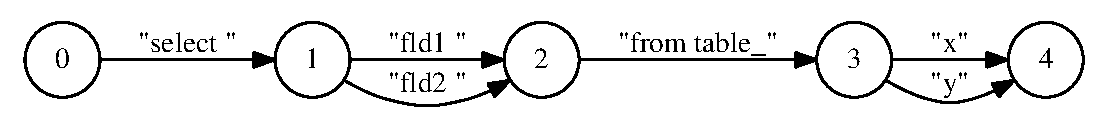
\includegraphics[scale=0.4]{graphs/lexer_example.eps}
    \end{center}
    \caption{Approximation for code presented in example 1}
    \label{lexer_input}
\end{figure}


The result of tokenization is presented in figure~\ref{tokens}. As far as we should preserve references to original code for tokens, we also demonstrate backreferences in this figure. {\bf Backreference} (br) is data on position of token in source code: corresponded string literals and position in literal. In the figure we present only corresponded literal data. Note that in simple case we can preserve only reference to source string literal, and for multipart literal we should preserve similar data for each part produced by each independent literal. Spaces and comments are skipped as in classical lexing.


\begin{figure}%[h!]
    \begin{center}
        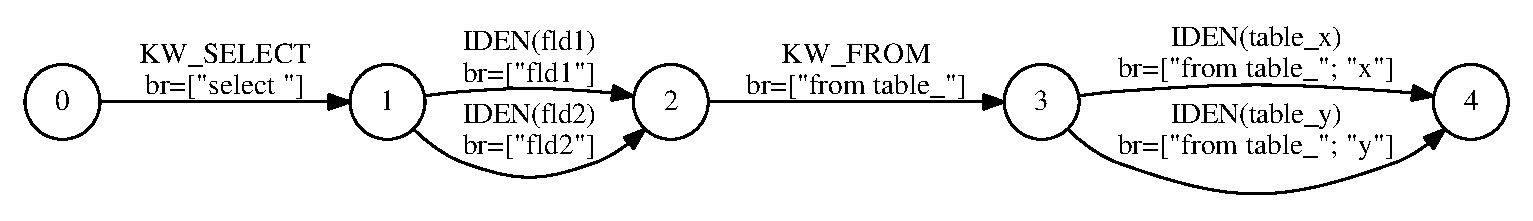
\includegraphics[scale=0.32]{graphs/lexer_example_tok.eps}
    \end{center}
    \caption{Result of graph presented in figure~\ref{lexer_input} tokenisation. Back references are shown.}
    \label{tokens}
\end{figure}



\subsection{Abstract Parser Generator}

Abstract parser generator based on RNGLR~\cite{RNGLR} passing algorithm was implemented as a part of YaccConstructor project. RNGLR is a modification of Tomita GLR algorithm~\cite{Tomita} which allows to process arbitrary context-free grammars. We use Yard language~\cite{YARD} as grammar specification language. Yard is a powerful language supporting Extended Backus-Naur Form, template rules and modularity. Also Yard supports attributed grammar specification, therefore it is possible to specify custom user semantic. 

Original GLR parsing algorithm can process {\it Shift/Reduce} and {\it Reduce/Reduce} conflicts~---~situations when available data are not enough to choose the correct way of parsing continuation. GLR analyses every possible way in case of conflict. This allows to produce several derivations for single input sequence. One may notice that processing of the linear subgraph does not differ from the processing of sequential input. In vertices with more than one outgoing edges the situation is similar to the classical LR conflict: there are several possibilities to Shift next token. This situation is not a conflict: all variants should be processed and there is no need to choose one of them, but we call this situation {\it Shift/Shift} conflict by the analogy with classical conflicts. {\it Shift/Shift} conflict processing produces new branches in stack as any classical conflict, so forks in input graph correspond to forks in GSS. Detailed description of modifications required to implement abstract parsing based on GLR parsing algorithm can be found in the paper~\cite{AGLR}.

We use classical graph structured stack and branch it when the fork appears in input graph. Unlike Alvor, we merge produced branches with equal states on the top: it improves performance and space requirements of algorithm. As far as we should process branches sequentially, we perform only single {\it push} for vertex with more than one outgoing edge at a time. {\it Push} corresponded with edge with minimal tail number in topological order should be performed immediately and other pushes should be postponed. Also we use shared packed parse forest (SPPF)~\cite{SPPF}~---~a compact representation of derivation forest which allows to reuse common nodes of derivation trees. This information is important for further discussion of error detection in abstract LR parsing.\newline 
    

\subsubsection{Error Detection and Error Recovery}

The result of classical parsing of sequential input in a case of no error recovery performed is either correct forest or error data. However, in abstract parsing we analyze the set of values: one value per each path in input graph. Therefore abstract parsing should return as an output the set of results: success or fail for each generated expression. The result of abstract syntactic analysis in our case is the list of detected errors for incorrect paths {\bf and} parse forest for all correct paths compressed into a single SPPF. Note that either error list or parse forest can be empty.

GLR parsing algorithm is targeted to ambiguous grammar processing and operates with graph structured stack which can be branched in case of conflict situation. The set of top vertices for every branch are {\it active vertices}~---~these vertices can be used for parsing continuation. In classical GLR if no action can be performed for some active vertex, then the vertex is removed from active vertices. Error is detected when the set of active vertices becomes empty. In abstract parsing it is a wrong approach. As far as stack branch can be produced not only by classical LR conflict but by the fork in input graph, impossibility of parsing continuation from the vertex may denote that the path being processed contains an error and corresponded data should be added to the result error set. Moreover, after an error has been detected in some path, parsing of other paths should be continued, but the processing of the erroneous paths should be skipped to prevent false error notifications. Current implementation of abstract parsing uses input graph vertex sequence sorted in the topological order as an input~\cite{AGLR} and this fact makes erroneous path eliminating rather nontrivial. When error is detected we should compute the set of vertices to skip. The next vertex to process can be selected either from postponed pushes or from active vertices. In the first case, the vertex with minimal tail number of postponed pushes should be chosen, and in the second~---~the vertex which can produce {\it push} to the vertex with minimal number. This way we skip only the subset of input graph edges which cannot be used in any correct paths. Figure~\ref{paths_ignoring} illustrates input edges skipping. The token \verb|")"| is erroneous, so edges $4 \to 6$ and $4 \to 5 \to 7$ should be skipped.

\begin{figure}[h!]
    \begin{center}
        \includegraphics[scale=0.4]{graphs/IgnoringPaths.pdf}
    \end{center}
    \caption{Example of paths skipping}
    \label{paths_ignoring}
\end{figure}

Note that error reporting and error recovery in Generalized LR parsing are nontrivial problems. A considerable amount of research has been done on improving error reporting for LR parsers, although for GLR parsers~\cite{GLROverview} relatively little work has been done. During the experiments we figured out that error processing in GLR-based abstract parsing is far more complex than in classical GLR parsing algorithm. It is caused by increased algorithm complexity (addition of a new type of conflict~---~{\it Shift/Shift}). So we should separate errors corresponded with wrong way of parsing continuation in classical LR conflicts and errors in the branches produced by {\it Shift/Shift} conflict. Conflicts mixing~---~when input grammar is ambiguous and input graph contains a lot of forks~---~is a situation in which the separation of actual errors and false errors produced by grammars ambiguity is nontrivial problem.

In spite of error recovery for RNGLR parsing algorithm has been implemented in YaccConstructor~\cite{GrigorevKirilenkoYC}, the necessity of its using in abstract parsing requires detailed research. Error recovery can be useful but it potentially produce a huge number of false errors for complex dynamic expressions.
    

\subsection{Semantic Calculation in Abstract Analysis}

Abstract parsing is based on GLR parsing algorithm and uses well-known structure to store parsing result (SPPF) which allows to calculate semantic for extracted trees. So it is possible to support user semantic calculation in abstract analysis in case when the attributed grammar is used for the language specification. But efficient tree extraction is a problem. Unlike classical GLR, SPPF in abstract parsing contains forest for multiple input values (all correct values of dynamically generated expression). When the number of possible values for expression is very big, a huge number of trees is extracted. Full parse forest extraction may require an exponential or even infinite memory. In the next sections we propose approaches aimed to decrease semantic calculation resource requirements, which we use in our tool.  

\subsubsection{SPPF Processing in Abstract Parsing}

Abstract parser returns parse forest compressed to SPPF which allows to share the nodes that are common for several parsing trees. In classical parsing nodes can be reused if they correspond to the same nonterminal and produce the same substring. Moreover, nonterminal may have more than one variant of derivation. Intermediate nodes represent such situations in SPPF: they allow to separate situations when nonterminal has multiple children (figure~\ref{s_childs}) and when nonterminal has several possible derivations (figure~\ref{2_derivations}). In our implementation intermediate nodes store information about the production which has caused the addition of the node to SPPF.

\begin{figure}[h!]
  \begin{center}
    \begin{subfigure}{0.2\textwidth}    
        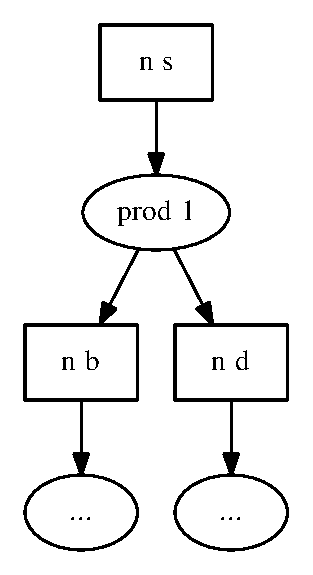
\includegraphics[scale=0.3]{graphs/SPPF_idea1.eps}    
    \caption{Nonterminal {\bf s} with multiple childs}
    \label{s_childs}
    \end{subfigure}
    ~
    \begin{subfigure}{0.2\textwidth}      
            \includegraphics[scale=0.3]{graphs/SPPF_idea2.eps}        
        \caption{Two different derivations  for nonterminal {\bf s}}
        \label{2_derivations}
    \end{subfigure}
    \caption{Node for rule $s \to b d$ (~\ref{s_childs}) and node for two different derivation for nonterminal s: $s \to b$ or $s \to d$ (~\ref{2_derivations}).}
    \label{sppf_idea}
  \end{center}
\end{figure}

Trees in abstract parsing often have big number of common nodes because different values of single dynamic expression usually have a big number of common parts. This makes SPPF a good option for parse forest of single dynamic expression compression. It is important fact that for every tree from SPPF there is correct expression generated by finite automaton, which approximates input.

Suppose it is not true: it means SPPF contains parse tree of expression which is not contained in approximation. Consider the following grammar.

\begin{verbatim}
s: a | b
a: A c
b: A D c
c: B | E F
\end{verbatim}

Let analyse a graph presented in figure~\ref{SPPF_proof_input}. Resulting SPPF should contain two trees: the derivation tree for sequence \verb|"AB"| and the other for sequence \verb|"ADEF"|. These trees are presented in figures~\ref{tree_sql_1} and ~\ref{tree_sql_2}. These two trees contain the node for nonterminal {\it c} and it seems that the trees can be merged as presented in figure~\ref{tree_sql_3}. In this case four trees can be extracted from resulted SPPF. They are derivation trees for input string \verb|"AB"|, \verb|"AEF"|, \verb|"ADB"|, \verb|"ADEF"|. But only two of them (\verb|"AB"| and \verb|"ADEF"|) can be generated by the input finite automaton.  

\begin{figure}[h!]
    \begin{center}
        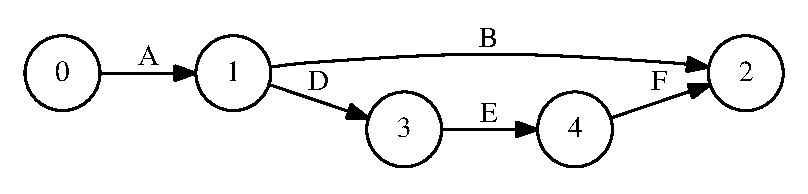
\includegraphics[scale=0.4]{graphs/SPPF_proof_input.eps}
    \end{center}
    \caption{Input graph which produces SPPF which contains multiple trees}
    \label{SPPF_proof_input}
\end{figure}
 
\begin{figure}[h!]
  \begin{center}
    	\begin{subfigure}{0.2\textwidth}    
    		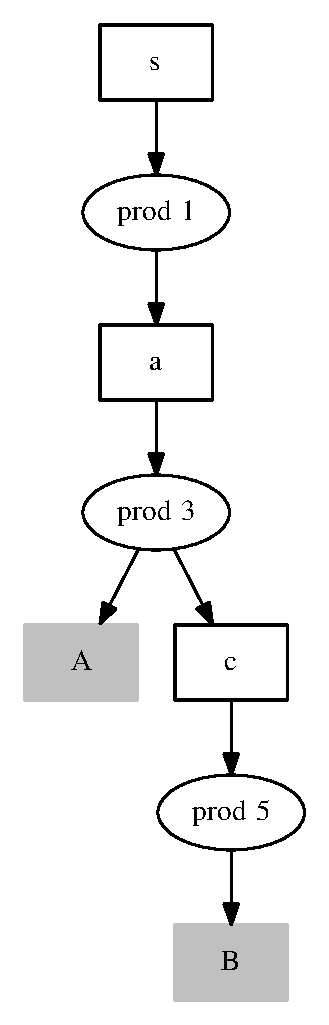
\includegraphics[scale=0.3]{graphs/SPPF_proof_fst.eps}    
    		\caption{First derivation tree}
    \label{tree_sql_1}
    \end{subfigure}
    ~
    \begin{subfigure}{0.2\textwidth}      
       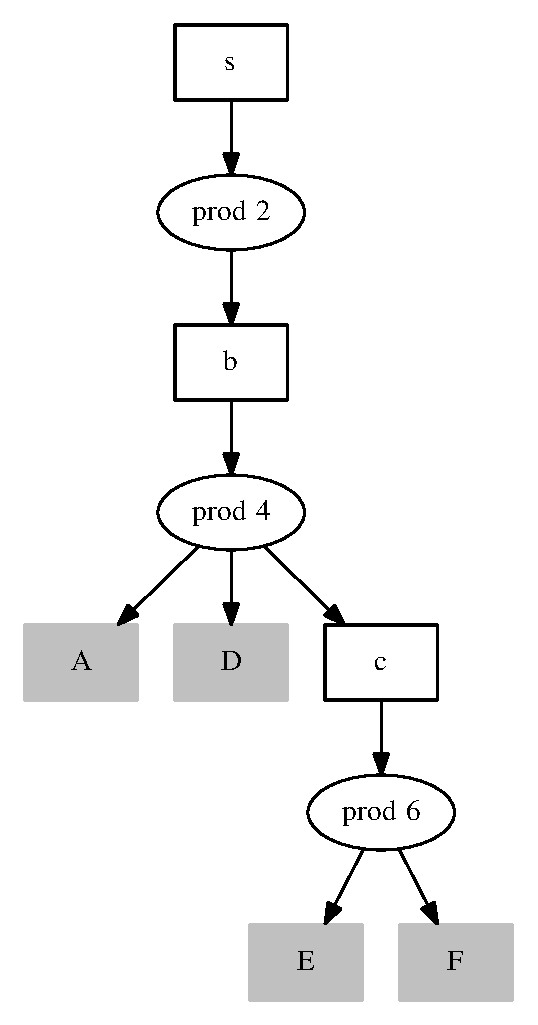
\includegraphics[scale=0.3]{graphs/SPPF_proof_snd.eps}
    
    	\caption{Second derivation tree}
    	\label{tree_sql_2}
    \end{subfigure}
    \\
    \begin{subfigure}{0.2\textwidth}      
       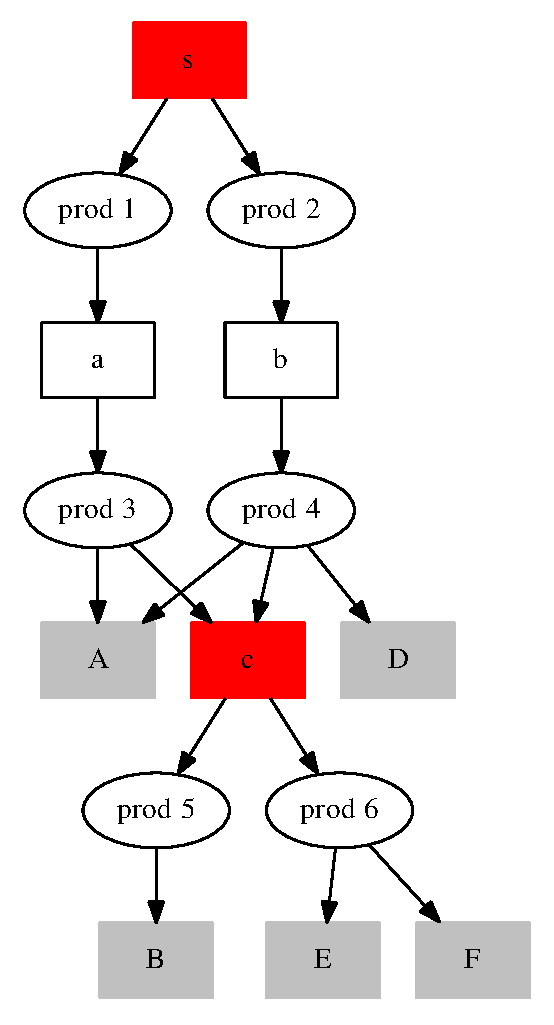
\includegraphics[scale=0.3]{graphs/SPPF_proof_incorrect.eps}    
    	\caption{Incorrect tree merging}
    	\label{tree_sql_3}
    \end{subfigure}
    ~
    \begin{subfigure}{0.2\textwidth}      
       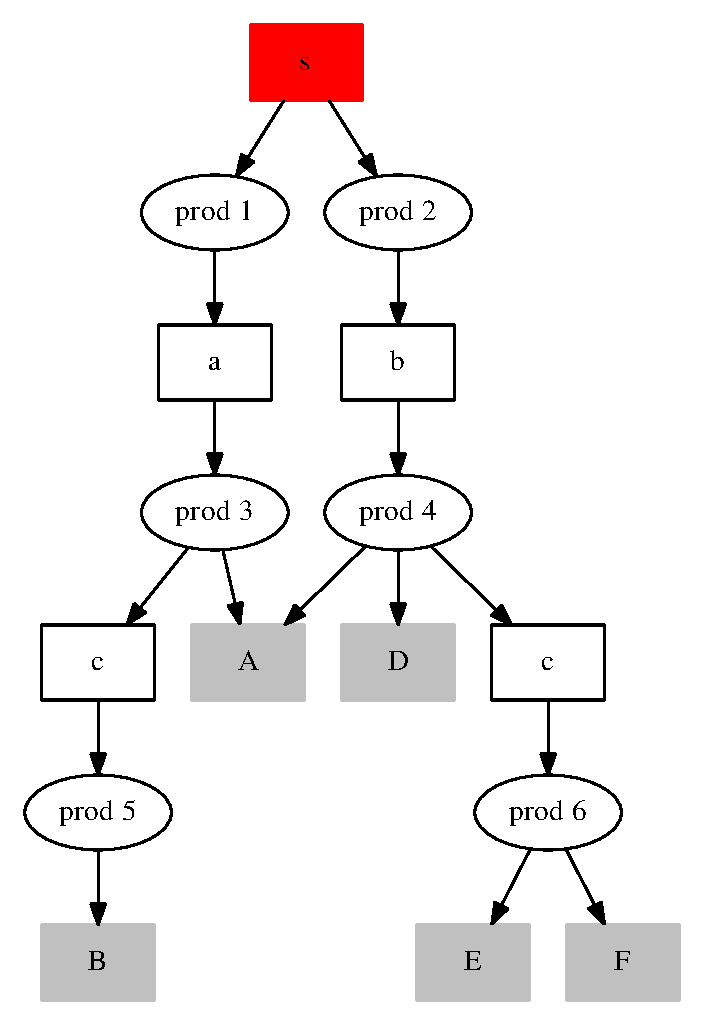
\includegraphics[scale=0.3]{graphs/SPPF_proof_correct.eps}    
    	\caption{Correct tree merging}
    	\label{SPPF_correct_merging}
    \end{subfigure}
    \caption{Tree merging}
    \label{trees_merging}
  \end{center}
\end{figure}


But it is not possible to get the SPPF presented in figure~\ref{tree_sql_3} because rules of merging are violated. Nodes can be reused only if derived substring are equal for both of them. But in our case one node for {\it c} is a derivation for string \verb|"B"| and the other node is a derivation for string \verb|"EF"|. We can not reuse this node for this reason. Only the node for terminal \verb|"A"| can be reused in our case. Corresponded SPPF is presented in figure~\ref{SPPF_correct_merging}. So if SPPF construction is correct~---~only nodes for actually common parts of expressions are reused~---~then SPPF does not contain incorrect trees.

\subsubsection{Syntax Highlighting}

It is not necessary to extract all the trees from SPPF for some tasks. For syntax highlighting, for example, it is enough to extract only a minimal subset of syntactically correct trees which contain all tokens in leaves. In other words, for every token we should extract at least one tree containing this token, and each tree usually contain more than one token which reduces the number of trees to be analysed. Textual representation of token in the source code can be colored in the single color, so even if there are two different trees, containing identical set of tokens, we use only one of them for code highlighting. Only one restriction is important: this tree should be syntactically correct. And this condition is always true because, as we discussed above, SPPF contains only correct trees.

\begin{figure}[h!]
    \begin{center}
        \includegraphics[scale=0.4]{graphs/sql_input_static_idea.eps}
    \end{center}
    \caption{Example of input for sql syntax highlighting}
    \label{sql_hl}
\end{figure}

A result SPPF for the input graph presented in figure~\ref{sql_hl} contains four trees. But two trees are enough for syntax highlighting. Remind that it should be trees containing all tokens from the graph. For example, the trees builded for the the next strings:  \verb|"SELECT age FROM tableName"| and \verb|"SELECT name FROM #table"|.

But it is still necessary to list all trees in the worst case: for instance, for the input graph presented in figure~\ref{bad_case}. Moreover, some algorithms may require full forest enumeration even for such graphs as one presented in figure~\ref{sql_hl}. 

\begin{figure}[h!]
    \begin{center}
        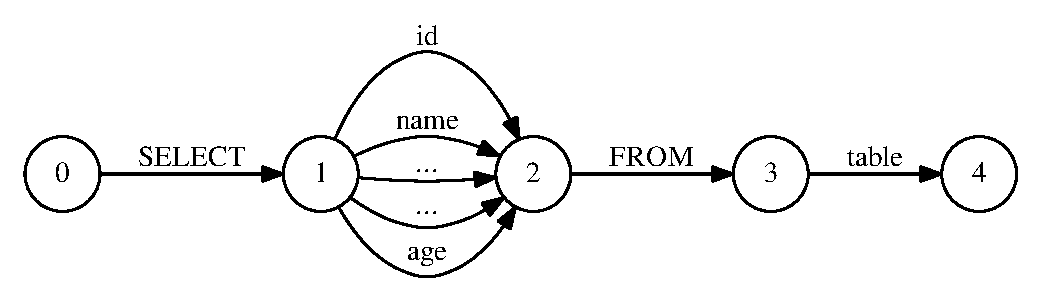
\includegraphics[scale=0.4]{graphs/Bad_case.eps}
    \end{center}
    \caption{An example of input graph which require enumerate all parsing trees}
    \label{bad_case}
\end{figure}


We propose lazy enumeration of trees to reduce time and memory consumption for semantics calculation. Lazy generation allows to start tree processing before the full forest is generated. Storing full forrest as a list of trees naturally leads to memory blowup, and lazy generation allows to avoid it. 

An algorithm of lazy tree generation may be implemented in different ways: it depends on the semantic calculation algorithms to be applied to parse trees. The tree enumeration algorithm which is usable for code highlighting is described below. The algorithm uses SPPF and context information~---~the set of tokens which are not contained in the list of already generated trees~---~to generate the next tree. 

To generate the next tree we traverse SPPF from the root. If vertex under consideration has more than one outgoing branch, we choose only one of possible derivation variants (one of subtree). Suppose we have two vertices in SPPF presented in figure~\ref{sppf_sql} where we should choose a subtree to include it in a result tree: vertex with label {\bf field} and vertex with label {\bf tableName}. Previously visited tokens are used to decide what tree should be chosen. This way, a subtree with biggest number of unvisited tokens are chosen. Consider the tree presented in figure~\ref{tree_sql_11} as a result of first traversal. When the next tree is extracted, there are two subtrees to choose from~---~containing token \verb|FIELD (age)| and containing token \verb|FIELD (name)|~---~in the vertex with label {\bf field}. But the token \verb|FIELD (age)| has been visited in the previous traversal and is contained in the first tree. Therefore the tree containing the token \verb|FIELD(name)| is chosen~\ref{tree_sql_22}.

In the case of multiple trees with equal number of unvisited tokens, any of the trees is chosen. Consider the tree presented in figure~\ref{tree_sql_11} as the first extracted tree. And suppose we try to process the vertex with label {\bf tableName} during the second tree generation. There are two possible subtrees and each of them contains only one token: \verb|TABLE(table2)| or \verb|TABLE(table3)|. At the current step we can choose any of these trees. There will be one more unvisited token after the step is completed, so one more traversal will be needed. The algorithm returns the next tree and the new set of unvisited tokens as a result. If the set of unvisited tokens is empty, then all required trees has been generated and empty tree is returned. 

\begin{figure}[h!]
    \begin{center}
        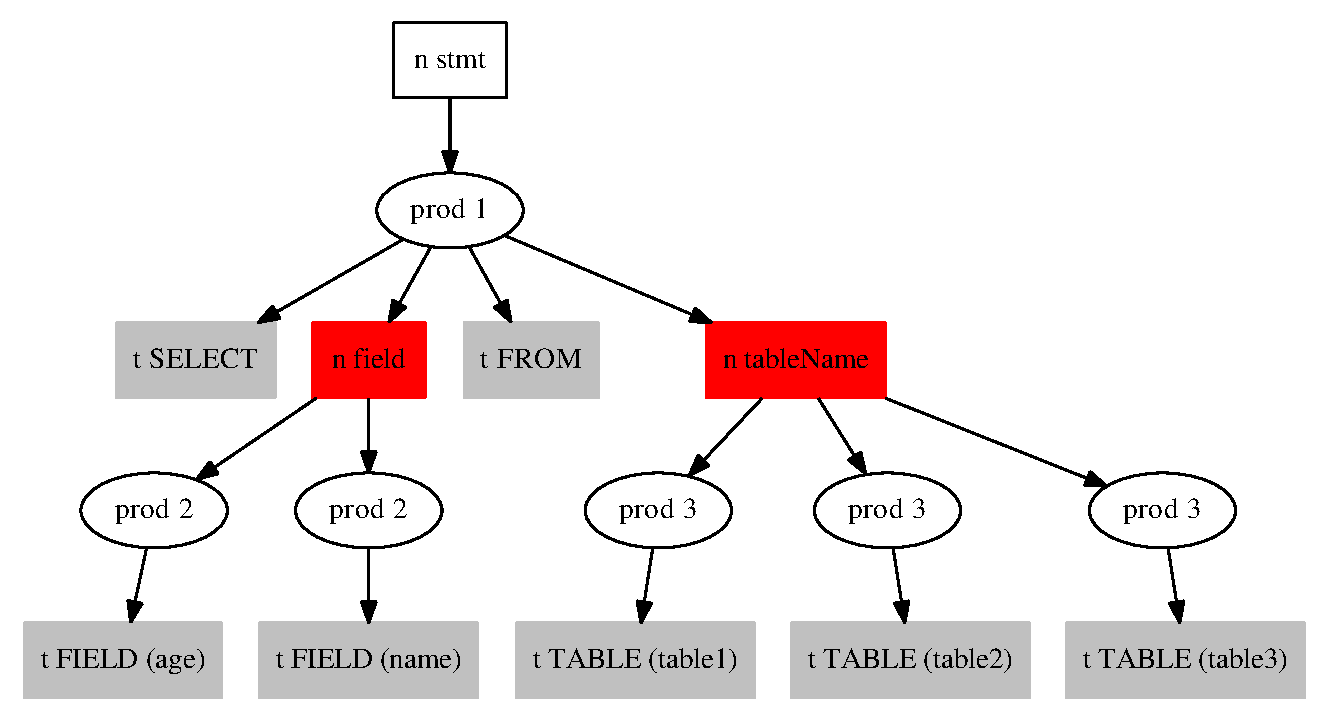
\includegraphics[scale=0.35]{graphs/SQL_sppf_static.eps}
    \end{center}
    \caption{Example of SPPF}
    \label{sppf_sql}
\end{figure}


\begin{figure}[h!]
  \begin{center}
    	\begin{subfigure}{0.2\textwidth}    
    		\includegraphics[scale=0.3]{graphs/SQL_sppf_static_tree1.eps}    
    		\caption{First tree}
    \label{tree_sql_11}
    \end{subfigure}
    ~
    \begin{subfigure}{0.2\textwidth}      
       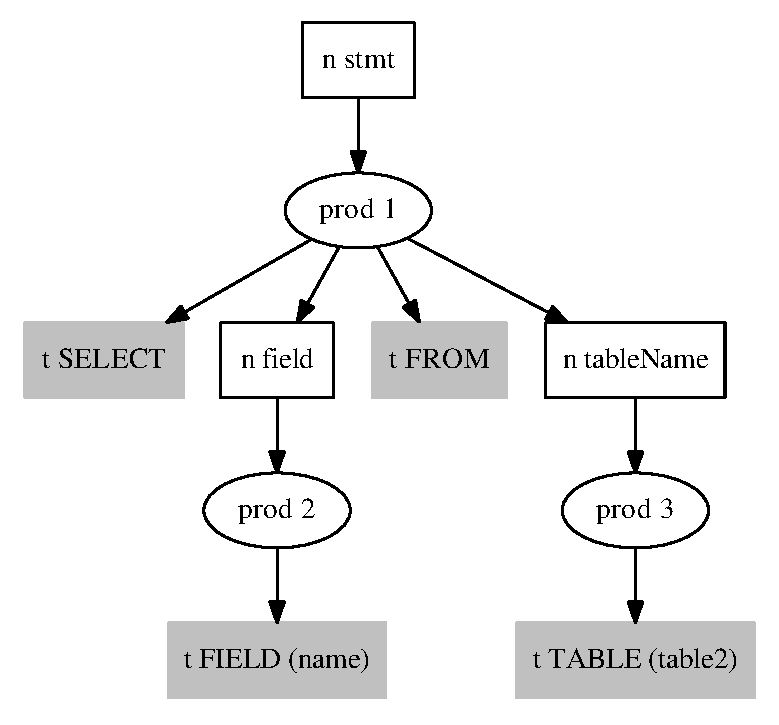
\includegraphics[scale=0.3]{graphs/SQL_sppf_static_tree2.eps}
    
    	\caption{Second tree}
    	\label{tree_sql_22}
    \end{subfigure}
    \\
    \begin{subfigure}{0.2\textwidth}      
       \includegraphics[scale=0.3]{graphs/SQL_sppf_static_tree3.eps}
    
    	\caption{Third tree}
    	\label{tree_sql_33}
    \end{subfigure}        
    \caption{Trees extracted from SPPF presented in figure~\ref{sppf_sql} }
    \label{trees_sql}
  \end{center}
\end{figure}

\subsubsection{Matching Delimiters Highlighting}

IDEs and code editors provide not only static code highlighting, but perform additional dynamic highlighting based on the context information. For instance, when the caret is placed before an opening parenthesis, the matching closing parenthesis is additionally highlighted. The similar feature is useful for string-embedded languages.

Consider the input graph presented in figure~\ref{insert_input}. Here we use \verb|LBR| and \verb|RBR| tokens to present left and right parentheses. Let the caret is placed just before the symbol which has been processed as \verb|LBR(1)|. As you can see, two different \verb|RBR| tokens match the selected \verb|LRB(1)|: \verb|RBR(1)| and \verb|RBR(2)|, so three symbols should be highlighted.  


\begin{figure*}
    \begin{center}
        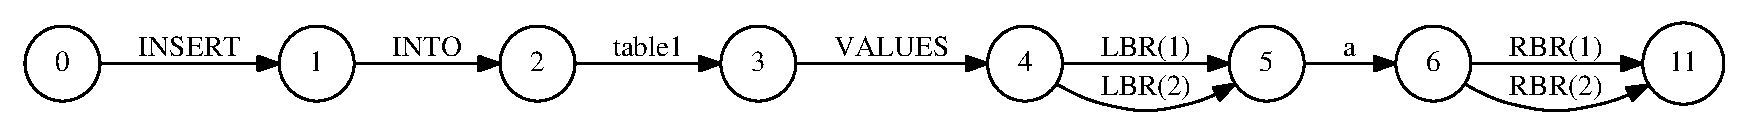
\includegraphics[scale=0.5]{graphs/insert_input.eps}
    \end{center}
    \caption{An example of input graph for delimiters highlighting}
    \label{insert_input}
\end{figure*}

Suppose, we have an algorithm for highlighting of matching delimiters for singular tree. In this case it is sufficient to enumerate the trees using the algorithm described above and apply existing matching delimiters highlighting algorithm. There is no need to enumerate all the trees for the matching delimiter highlighting~---~we can filter them by the existence of the matching token.

\section{Evaluation}

The platform described above is implemented in F\#~\cite{FS} programming language and named {\bf AbstractYaccConst-ructor}~---~AYC.  AYC is a part of YaccConstructor~---~grammarware research and development project. Plug-in to Microsoft Visual Studio IDE based on ReSharper is also implemented. This plug-in is created as a demonstration of AYC and at the same time is a tool for supporting string-embedded languages in Microsoft Visual Studio IDE.

We has implemented plug-ins for two languages: arithmetic expression language (named {\bf Calc}) and the subset of T-SQL language. We has developed lexer and parser specifications for this languages. Lexer specification was developed in a subset of FsLex language which is supported by the abstract lexer generator. Grammar (parser specification) was written in Yard language. The set of specifications can be find in the project repository\footnote{YaccConstructor source code  (accessed: 07.07.2014):\url{https://code.google.com/p/recursive-ascent/}}. These specifications has been used for abstract lexer and abstract parser generation using generators described above. XML-files for syntax highlighting specification and the set of classes for integration with ReSharper has been also produced during parser generation. Finally, we has built a package for each language using generated stuff. 

Built  packages has been loaded into the plug-in to demonstrate features provided by them. In the current version you should specify {\bf hotspot methods}~---~methods which can process string-embedded languages~---~and corresponded languages in special configuration file to get an ability to define mapping from string literals to languages. 

We have created test project and have defined hotspot methods for our string-embedded languages: {\it ExecuteImmediate} for T-SQL and {\it Eval} for Calc language. We present examples of functionality of created language extensions below.

{\bf Syntax highlighting.} Example of string-embedded T-SQL syntax highlighting is presented in the figure~\ref{sqlHighlighting}. Only keywords are highlighted in the current configuration. One can easily configure colors for different token types using configuration XML-file generated automatically for highlighting customization. You can see that multipart tokens are supported correctly: the insert keyword is built from two string literals, and it is still detected as keyword and highlighted properly. You can also see that in the figure~\ref{languages} in the line 14 \verb|"where"| substring is not a keyword, although it may seem so if the first literal is analysed separately. But if the whole statement is analysed, we detect that it is an identifier \verb|"wherev"|, so it should not be highlighted as a keyword.
  

\begin{figure}[h!]
    \begin{center}
        \includegraphics[scale=0.3]{graphics/Insert.png}
    \end{center}
    \caption{T-SQL syntax highlighting}
    \label{sqlHighlighting}
\end{figure}
 
{\bf Multiple languages support.} An example of multiple string-embedded languages support is presented in the figure~\ref{languages}. You can see that highlighting can be configured independently: numbers in T-SQL and in Calc expressions have different color.

\begin{figure}[h!]
    \begin{center}
        \includegraphics[scale=0.3]{graphics/Languages.png}
    \end{center}
    \caption{Multiple language support}
    \label{languages}
\end{figure}

{\bf Static errors detection and notification.} Our plug-in provides static error detection for string-embedded languages. You can see an example of this feature in the figure~\ref{languages} in line 13: an error in values to insert is detected. An important feature of our algorithm is an ability to detect multiple errors: one error for each possible value of dynamic expression can be found. For example, the string to be executed can construct two different values by means of {\it if}-statement and every branch contains an error (figure ~\ref{staticErrors}). All these errors are found in such case by our tool unlike Alvor which detects only one error in the similar test described above (Figure~\ref{ex_alvor}).

\begin{figure}[h!]
    \begin{center}
        \includegraphics[scale=0.3]{graphics/Select_like_Alvor_example.png}
    \end{center}
    \caption{Static error detection}
    \label{staticErrors}
\end{figure}

{\bf Matching parenthesis highlighting.} The feature which significantly improves readability and understanding of the code is matching parenthesis highlighting: if the caret is placed near one  of the parenthesis, then the tool should highlight the matching parenthesis. This feature is also useful for string-embedded languages but its implementation is more complex than in classical languages analysis. The construction of an expression using string-embedded language is more flexible, so several matching elements may exist for the selected one. You can see such situation in the figure~\ref{brace1}: there are two closing parentheses (in line 12 and 14) for the selected opening one (line 10), so all three symbols are highlighted. On the other hand, there are only one left parenthesis for each right one. So, if we select right parenthesis in line 14 then only one left parenthesis is highlighted (Figure~\ref{brace2}). There are special section in highlighting configuration XML-file where the matching delimiters can be specified.


\begin{figure}[h!]
  \begin{center}
    \begin{subfigure}[t]{0.2\textwidth}    
        \includegraphics[scale=0.25]{graphics/bracket_1.png}    
    \caption{Multiple matches}
    \label{brace1}
    \end{subfigure}
    ~
    \begin{subfigure}[t]{0.2\textwidth}      
            \includegraphics[scale=0.25]{graphics/bracket_3.png}        
        \caption{Single match}
        \label{brace2}
    \end{subfigure}
    \caption{Paranthesis highlighting}
    \label{braces}
  \end{center}
\end{figure}

We have demonstrated a possibility of separated implementation of support for different string-embedded languages based on SDK and the plug-in described above. Provided functionality are presented. We can conclude that even though at the current moment functionality completeness is lower than in similar tools, our tool can process more complex cases: branches and concatenations are supported, multiple errors can be found, highlighting is configurable.


\section{Future Work}

Improvements in both the platform and the plug-in are necessary. At the platform level, it is necessary to implement mechanisms required for string-embedded language. Embedded language transformation may be useful for system migration from one DBMS to another~\cite{GrigorevDSQL} or for migration to new techniques such as LINQ. This task corresponds with two big problems: possibility of nontrivial transformations (some advanced techniques~\cite{Ter1,Bou_Ko} may be useful for this problem) and transformation correctness proof. An approximation also requires improvement. First of all, we should support cycles in input graph for abstract lexing and abstract parsing. The composition of two FST is also FST~\cite{FST}. So string operations which can be described with FST (replace, trim, substring, remove, etc.) can be supported naturally at abstract lexer step. 

The next big task is error detection and notification improvement. The main direction of research here is a migration to abstract parsing based on GLL parsing algorithm. Motivation is that the quality of error processing is higher in LL-parsers than in LR and implementation is simplier. If this characteristics are inherited in abstract GLL~\cite{GLL}, then the error processing in abstract parsing will be improved. We are also going to implement type checking for string-embedded languages. For SQL it may be type checking inside the dynamically constructed queries and the consistency of returned and expected types: we should check whether the type of query result equals to the type of the variable to which the result is assigned.


%Список литературы
%Кириленко Я.А., Григорьев С. В.,Авдюхин Д. А.: Разработка синтаксических анализаторов в проектах по автоматизированному реинжинирингу информационных систем. Научно-технические ведомости СПбГПУ информатика, телекоммуникации, управление. Номер: 174, 2013 — 94-98
%	ReSharper. URL: http://www.jetbrains.com/resharper/
%Microsoft Visual Studio. URL: http://www.visualstudio.com
%Kyung-Goo Doh, Hyunha Kim, and David A. Schmidt: Abstract parsing: Static analysis of dynamically generated string output using lr-parsing technology. In Proceedings of the 16th International Symposium on Static Analysis, SAS ’09. Springer-Verlag: Berlin; Heidelberg, 2009. P. 256–272.
%Aivar Annamaa, Andrey Breslav, and Varmo Vene: Using abstract lexical analysis and parsing to detect errors in string-embedded dsl statements. In Marina Walden and Luigia Petre, editors, Proceedings of the 22nd Nordic Workshop on Programming Theory.
%Java String Analyzer.  URL: http://www.brics.dk/JSA/.
%Alvor. URL: http://code.google.com/p/alvor/.
%PHP string analyzer.  URL: http://www.score.is.tsukuba.ac.jp/~minamide/phpsa/.
%Mohri Mehryar: Finite-State Transducers in Language and Speech Processing. Association for Computational Linguistics. ― 1997. ― http://www.cs.nyu.edu/ mohri/pub/cl1.pdf
%Вербицкая E.A., Григорьев С.В.  Абстрактный лексический анализ  СПИСОК-2013: Материалы всероссийской научной конференции по проблемам информатики. 23–26 апр. 2013 г., Санкт-Петербург. — СПб.: Издательство ВВМ, 2013 792 с.
%Elizabeth Scott and Adrian Johnstone. 2006. Right nulled GLR parsers. ACM Trans. Program. Lang. Syst. 28, 4 (July 2006), 577-618. 
%GLR-based abstract parsing: http://dl.acm.org/citation.cfm?id=2556616&dl=ACM&coll=DL
%Syrcose-шная: From Abstract Parsing to Abstract Translation http://syrcose.ispras.ru/2014/files/SYRCoSE2014_Proceedings.pdf
% A. S. Christensen, A. Møller, and M. I. Schwartzbach. Precise analysis of string expressions. In Proceedings of the Static Analysis Symposium (SAS), volume 2694 of LNCS, pages 1–18, 2003.
%http://www.score.cs.tsukuba.ac.jp/~minamide/papers/www05.pdf Строковые операции с помощью FST



%
% The following two commands are all you need in the
% initial runs of your .tex file to
% produce the bibliography for the citations in your paper.
\bibliographystyle{abbrv}
%\bibliography{sigproc}  % sigproc.bib is the name of the Bibliography in this case

\begin{thebibliography}{}

\bibitem{ALVOR1}
Annamaa A., Breslav A., Kabanov J. e.a. An Interactive Tool for Analyzing Embedded SQL Queries. Programming Languages and Systems. LNCS, vol. 6461. Springer: Berlin; Heidelberg, p. 131--138, 2010.

%\bibitem{ALVOR2}
%Annamaa A., Breslav A., Vene V. Using Abstract Lexical Analysis and Parsing to Detect Errors in String-embedded DSL Statements, Proceedings of the 22nd Nordic Workshop on Programming Theory. Marina Walden and Luigia Petre, editors, p. 20--22. 2010.

%\bibitem{AbstrParsing}
%Kyung-Goo Doh, Hyunha Kim, David A. Schmidt. Abstract Parsing: Static Analysis of Dynamically Generated Sring Output Using LR-parsing Technology, Proceedings of the 16th International Symposium on Static Analysis, SAS’09. Springer-Verlag: Berlin; Heidelberg, p. 256--272, 2009.

\bibitem{LRAbstrParsing}
Kyung-Goo Doh, Hyunha Kim, and David A. Schmidt. Abstract LR-parsing, In Formal modeling, Gul Agha, Jos{\'e} Meseguer, and Olivier Danvy (Eds.). Springer-Verlag, Berlin, Heidelberg, p. 90--109, 2011.

%\bibitem{LRAbstrParsingSema}
%H. Kim, K. Doh,  and D.A. Schmidt,  Static Validation of Dynamically Generated HTML Documents Based on Abstract Parsing and Semantic Processing.;In Proceedings of SAS, 194 -- 214, 2013.

\bibitem{GLL}
Elizabeth Scott and Adrian Johnstone. 2010. GLL Parsing, Electron. Notes Theor. Comput. Sci. 253, 7 (September 2010), p. 177--189. 

\bibitem{SPPF}
Rekers J. G. 1992. Parser generation for interactive environments. Ph.D. thesis, Universty of Amsterdam.

%\bibitem{Grune}
%Grune D., Ceriel J. H. Jacobs. Parsing techniques: a practical guide. Ellis Horwood, Upper Saddle River, NJ, USA, 1990. p. 322.

\bibitem{GrigorevKirilenkoYC}
Iakov Kirilenko, Semen Grigorev, and Dmitriy Avdiukhin. Syntax analyzers development in automated reengineering of informational system.
St. Petersburg State Polytechnical University Journal. Computer Science. Telecommunications and Control Systems, 174(3), June 2013.

\bibitem{Minamide}
Yasuhiko Minamide. Static approximation of dynamically generated web pages. In Proceedings of the 14th International Conference on World
  Wide Web, WWW '05, p. 432--441, New York, NY, USA, 2005. ACM.

\bibitem{RNGLR}
Elizabeth Scott and Adrian Johnstone. Right nulled glr parsers. ACM Trans. Program. Lang. Syst., 28(4):p. 577 -- 618, July 2006.

\bibitem{StringExpr}
Aske Simon Christensen, M{\o}ller A., Michael I. Schwartzbach. Precise analysis of string expressions, Proc. 10th International Static Analysis Symposium (SAS), Vol. 2694 of LNCS. Springer-Verlag: Berlin; Heidelberg, June, p. 1 -- 18, 2003.


%\bibitem{SAofStrVal}
%Costantini G., Ferrara P., Cortesi F. Static analysis of string values, Proceedings of the 13th international conference on Formal methods and software engineering, ICFEM’11. Springer-Verlag: Berlin; Heidelberg, p. 505-521, 2011.


%\bibitem{ISO}
%ISO. ISO/IEC 9075:1992: Title: Information technology~---~Database languages~---~SQL. 1992. p. 668.

%\bibitem{SAForInject}
%Xiang Fu, Xin Lu, Peltsverger B. e.a. A static analysis framework for detecting SQL injection vulnerabilities, Proceedings of the 31st Annual International Computer Software and Applications Conference. Vol. 01, COMPSAC '07, Washington, DC, USA, IEEE Computer Society, p. 87--96, 2007.

%\bibitem{Dasgupta}
%Arjun Dasgupta, Vivek Narasayya, and Manoj Syamala. A static analysis framework for database applications. In Proceedings of the 2009 IEEE International Conference on Data Engineering, ICDE '09, p. 1403--1414, Washington, DC, USA, 2009. IEEE Computer Society.

\bibitem{GrigorevDSQL}
Semen Grigorev. Automated transformation of dynamic sql queries in information system reengineering. Master's thesis, Saint-Petersburg State University, 2012.

\bibitem{YARD}
Dmitry Avdyukhin. Translation definition language for informational system reengineering tools. Graduation thesis, Saint-Petersburg State University, 2013.


\bibitem{GLROverview}
 Giorgios Robert Economopoulos. Generalised LR parsing algorithms. 2006.
 
\bibitem{Tomita} 
 Tomita, Masaru. LR parsers for natural languages, In 10th International Conference on Computational Linguistics, p. 354--357. ACL, 1984.

%\bibitem{AbstractInterpretation} 
% Patrick Cousot and Radhia Cousot. 1977. Abstract interpretation: a unified lattice model for static analysis of programs by construction or approximation of fixpoints. In Proceedings of the 4th ACM SIGACT-SIGPLAN symposium on Principles of programming languages (POPL '77). ACM, New York, NY, USA, p. 238--252.
 
\bibitem{FS}
Syme D., Granicz A., and Cisternino A.: Expert F\#, Apress (2007).

%\bibitem{BRNGLR}
%Elizabeth Scott, Adrian Johnstone, and Rob Economopoulos. 2007. BRNGLR: a cubic Tomita-style GLR parsing algorithm. Acta Inf. 44, 6 (September 2007), p. 427-461.

%\bibitem{RIGLR}
%Elizabeth Scott and Adrian Johnstone. Table based parsers with reduced stack activity. Technical Report CSD-TR-02-08, Royal Holloway, University of London, Department of Computer Science, Egham, Surrey TW20 0EX, England, May 2003.

\bibitem{AGLR}
Semen Grigorev and Iakov Kirilenko. 2013. GLR-based abstract parsing. In Proceedings of the 9th Central \& Eastern European Software Engineering Conference in Russia (CEE-SECR '13). ACM, New York, NY, USA, Article 5, 9 pages.

\bibitem{Ter1}
Andrey Terekhov. 2013. Good technology makes the difficult task easy. In Proceedings of the 2013 9th Joint Meeting on Foundations of Software Engineering (ESEC/FSE 2013). ACM, New York, NY, USA, P. 683--686.

\bibitem{Bou_Ko}
D. Yu. Boulychev, D. V. Koznov, and Andrey A. Terekhov. 2002. On Project-Specific Languages and Their Application in Reengineering. In Proceedings of the 6th European Conference on Software Maintenance and Reengineering (CSMR '02). IEEE Computer Society, Washington, DC, USA, p. 177--185.

\bibitem{FST}
Mehryar Mohri. 1997. Finite-state transducers in language and speech processing. Comput. Linguist. 23, 2 (June 1997), p. 269--311.


\end{thebibliography}

\balancecolumns


% That's all folks!
\end{document}
